\section{Introduction}

In recent years, the rise of commission-free trading platforms has profoundly reshaped retail investor behavior and sparked growing interest among scholars in behavioral finance. 
One of the most prominent examples is Robinhood, a mobile-first brokerage that gained widespread popularity for eliminating trading fees and offering a highly gamified user experience. 
The platform attracted a large number of retail investors, particularly young and inexperienced individuals\footnote{
According to Robinhood's IPO filing, the typical user on the platform is 31 years old, with an average account balance of approximately \$3,500. 
Notably, around half of the platform's users are investing for the first time.}.

An important development in the empirical literature was the release of Robintrack, an open-source dataset that tracks the number of Robinhood users holding individual stocks over time. 
This data, collected via Robinhood's public API, provides a rare opportunity to directly observe the trading dynamics and portfolio shifts of real retail investors. 
The dataset can be downloaded from \url{https://robintrack.net/}.

Several recent studies, including \cite{Fedyk2024} and \cite{Welch2022}\footnote{it must be noted that the former explicitly follows the method of the latter}, 
have leveraged the Robintrack dataset to examine retail investor performance. 
Their findings suggest that Robinhood investors, contrary to popular belief, exhibited strong market timing and outperformed passive benchmarks. 
In particular, these papers report significant cumulative returns and positive alpha using standard factor models.

In this paper, we revisit these claims by constructing an alternative methodology for portfolio formation based on the same dataset. 
Specifically, we analyze whether the returns of Robinhood users' favorite stocks exhibit stochastic dominance over benchmark indices.
Our goal is to offer a more nuanced assessment of whether retail investors truly generate abnormal returns or whether previous results may be driven by sample selection or methodological choices.

\subsection{Literature Review}

The literature on retail investor performance has evolved considerably over the past two decades. 
Early foundational work highlighted persistent underperformance by individual investors, while more recent studies leveraging novel, high-frequency data sources have painted a more nuanced picture, one in which method choice can swing conclusions from "retail crowd outperforms" to "retail crowd underperforms."
This paper introduces a novel approach in studying directly investor performance, while drawing insights on the risk aversion to assess the relaibility of the collected data and possible behavioral biases.

The canonical starting point to analyse trading and behavioral biases is the seminal work of \cite{BarberOdean2000}. 
Using account-level brokerage records, they show that individual investors engage in trading with excessive frequencey, incurring higher transaction costs, 
exhibiting poor timing. This ultimately leads to underperformance relative to buy-and-hold benchmarks.
The main message of their study is in the title of the paper itself, "Trading Is Hazardous to Your Wealth".  
In their analysis of individual trading accounts from an important broker, they find that the most active accounts underperform the market by approximately 6.5\% per year, net of fees. 
This result firmly establishes that behavioral biases such as overconfidence, turnover, and attention-driven trading harm returns of retail participants.
Moreover, \cite{Grinblatt2001} use Finnish account-level data, documenting several behavioral biases in  their trading patterns.
They show evidence of investors being reluctant to realize losses and that hat trading intensity rises following past returns and when stocks reach monthly highs or lows.

Building on advances in data availability, \cite{Welch2022} and \cite{Fedyk2024} both exploit the Robintrack dataset to construct a "Robinhood crowd" portfolio, 
althoug focusing only on U.S. common stocks.
\cite{Welch2022} introduces two weighting schemes identical to those later used by Fedyk, and documents that, when building a portfolio with yesterday's crowd-popularity weights to today's returns, the resulting performance has significant positive alpha over the February 2018-August 2020 sample. 
The aggregate Robinhood portfolio earned an average six-factor daily alpha of 6.5 basis points.
Remarkably, retail investors appear to have timed the market successfully, outperforming a U.S. stock index while achieving similar drawdowns.

\cite{Fedyk2024} closely follows Welch's methodology, aggregating hourly Robintrack counts into daily weights and applying a one-day lag to avoid look-ahead bias. 
She confirms Welch's core finding of very high positive returns and documents robustness across factor models. 
Importantly, Fedyk also compares the "dollar" versus "share" weighting schemes and shows that both yield similar outperformance.
The author also decomposes the returns through three behavioral channels.
A "buy-the-dip" effect is particularly pronounced in large-cap stocks, showing positive excessive returns in the very-short terms.
Robinhood investors also show more activity around announcements and analyst recommendation revisions,
and attention spilloveers driven by WallStreetBets sentiment. 

\cite{ardia2023fastfurioushighfrequencyanalysis} leverage higher frequency data to reveal that Robinhood users exhibit a high-frequency, contrarian trading style:
Robinhood investors disproportionally buy big losers within an hour of extreme negative returns and show higher sensitivity to overnight moves.

The literature in behavioral finance highlights the importance of limited attention and the importance of information.
\cite{barber2021robinhood} also make use of the robintrack dataset to show that Robinhood users engage in extreme attention-induced herding episodes.
Notably, these episodes are followed by large negative returns.
They document that this herding behavior is driven by Robinhood's "Top Mover" interface, highlighting the importance of gameification in shaping investors preferences. 
\cite{zhi2009} show that increases in the Google Search Volume Index for a given ticker are correlated with investing activity of retial investors.
In addition to this, increased retail attention can explain the long run underperformance of IPO stocks.
Beyond raw attention effects, interface design and social media contagion further shape retail behavior.
\cite{semenova2023socialcontagionassetprices} use Reddit's WallStreetBets discussions to show that peer-driven cascades amplify price momentum and reversals,
as traders coordinate through social network to drive short-term bubbles.

%%%%%
In sum, the existing literature vividly illustrates that retail-investor performance hinges critically on both measurement design and behavioral dynamics
Yet, a cohesive framework that emebeds risk aversion considerations remains absent.
This paper fills the gap by evaluating the performance of retail investors not only through risk-adjusted and raw returns but also 
through CRRA utility estimation, allowing us to compute welfare losses retail investors incur when behavioral biases misalign their portfolios.
Stochastic dominance tests are also presented, supporting a less beenvolent view of Robinhood investors and raising a question of rationality.
In doing so, we provide a cohesive assesment of behavioral drivers of returns and risk aversion implied by revealed preferences,
offering a more structurally consistent and behaviorally meaningful evaluation of whether and how "the wisdom of the crows" truly materializes.

\subsection{Description of the Robinhood Dataset}
The dataset records the number of Robinhood users holding at least one share of 8,619 securities, with observations taken hourly. 
Following \cite{Welch2022} and \cite{Fedyk2024}, we aggregate this data on a daily basis by selecting the last observation of each trading day.

The sample spans from February 5, 2018, to August 13, 2020, covering 818 days. Note that the dataset includes non-trading days and contains some missing observations.

Since the dataset only provides the number of investors per security, we cannot track individual holdings, monetary amounts, or share quantities. 
Moreover, buy/sell flows are unobservable; however, we can approximate them using changes in the number of holders.

We merge this dataset with CRSP to obtain market-level information and later construct a benchmark index. 
The resulting dataset contains 7,613 unique securities, substantially more than in \cite{Fedyk2024} and \cite{Welch2022}, who restrict their analysis to U.S. common stocks only. 
The original Robinhood dataset contains missing observations for 3,331 securities, predominantly in the earlier sample periods. 
Following \cite{Fedyk2024}, we therefore construct the Robinhood portfolio on a daily basis using only those securities with available price data; 
any security lacking a quote on a given date is excluded from that day's portfolio. 
Additionally, we exclude all securities identified as problematic in their appendix. 

In terms of security types, common stocks represent 57.3\% of the dataset, while ETFs and other funds account for 26.3\% and 8.7\%, respectively. 
Structured products, REITs, and ADRs constitute the remaining share. 
When classifying by market capitalization, stocks dominate with 83.1\%, followed by ETFs (9.3\%) and other funds (3.3\%).

The total number of open positions on any given day is calculated as the sum of users holding at least one share across all securities, i.e., a row-wise sum across the dataset.

Market data for each security was retrieved from CRSP\footnote{The Center for Research in Security Prices (CRSP), based at the University of Chicago, provides high-quality historical market data widely used in finance research and investment analysis.} via WRDS. 
Out of the full universe, 8,099 securities were available in CRSP, as it includes only U.S.-listed assets. 


\begin{figure}[H]
    \centering
    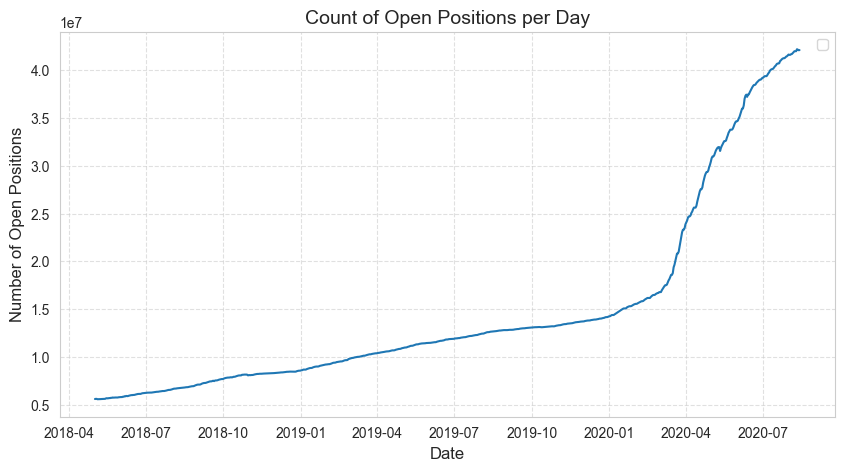
\includegraphics[width=1\linewidth]{../images/old/no_positions_date.png}
    \caption{Daily count of open Robinhood positions, May 2018-August 2020.}
\end{figure}

The figure above shows the daily count of open positions on Robinhood from April 2018 to mid-2020. 
We observe a steady increase in user participation, with a sharp acceleration beginning in early 2020. 
This surge coincides with the onset of the COVID-19 pandemic, likely driven by a combination of heightened market volatility, increased retail interest, and fiscal stimulus payments.
